\documentclass{article}
\usepackage{graphicx} 
\usepackage{float}
\usepackage{booktabs}
\usepackage{array}
\usepackage{arydshln}
\usepackage{siunitx}
\usepackage{cancel}
\usepackage{changepage}
\usepackage{placeins}
\usepackage{enumitem}
\usepackage{siunitx}
\usepackage{lipsum}
\usepackage[most]{tcolorbox}
\definecolor{light-gray}{gray}{0.9}
\newcommand{\code}[1]{\colorbox{light-gray}{\texttt{#1}}}
\usepackage{subcaption}

\usepackage{parskip}
\usepackage{times}
%\usepackage{mathpazo}
%\usepackage{tgtermes}

\DeclareSIUnit{\atm}{atm}

\usepackage{tabularx}
\usepackage{amsmath, amssymb, amscd, MnSymbol, mathrsfs}
\usepackage{cellspace}
\usepackage{tikz}
\usetikzlibrary{calc,3d, patterns, angles, quotes, decorations.markings, decorations.pathmorphing, hobby}
\usepackage{xfrac}

\usepackage{chemfig}
\usepackage{caption}
\usepackage{bm}

\usepackage{pdfpages}
\usepackage{pdflscape}
\usepackage{afterpage}

\usepackage{empheq}
\usepackage{pgfplots}
\usepackage{pgfplotstable}
\usepackage{xstring}

\pgfplotsset{compat=1.18}


\usepackage[european,americanvoltages,americanresistors,cuteinductors,fetbodydiode]{circuitikz}
\usetikzlibrary{circuits.logic.US}
\usepackage{siunitx}
\usetikzlibrary{arrows,shapes,calc, positioning, patterns, decorations, decorations.markings}
\usetikzlibrary{positioning}
\usetikzlibrary{calc}
%\ctikzset{bipoles/thickness=1}
%\tikzstyle{every node}=[font=\small]
%\tikzstyle{every path}=[line width=0.8pt,line cap=round,line join=round]

\def\CalcC#1{%
	\coordinate (base) at (#1.base);
	\coordinate (collector) at (#1.collector);
	\coordinate (emitter) at (#1.emitter);
	\draw (barycentric cs:base=0.5,collector=0.5,emitter=0.5) circle [radius=14pt];
}

\usepackage{tikz-3dplot}
\usepackage{textcomp}
% Custom commands
\newcommand{\vect}[1]{\boldsymbol{\mathbf{#1}}}
\newcolumntype{C}{>{\centering\arraybackslash}X}
\newcolumntype{M}[1]{>{\centering\arraybackslash}m{#1}}

%\usetikzlibrary{external}
%\tikzexternalize[prefix=figures/]

\newcommand\myfrac[2]{\sfrac{#1\mkern-1.2mu}{#2}}
\usepackage{xcolor}

% Define custom colors
\definecolor{darkblue}{rgb}{0.1,0.1,0.5} %  dark blue shade
\definecolor{formalshade}{rgb}{0.95,0.95,1} % light blue shade for the background

% For the adjustwidth environment
\PassOptionsToPackage{strict}{changepage}
\usepackage{changepage}

% For formal definitions

\usepackage{framed}
\newcommand{\formalsource}{}

\newenvironment{formal}[3][]{	\renewcommand{\formalsource}{#1}
	\def\lefty{\color{#2}\textquotedblleft}
	\def\righty{\color{#2}\textquotedblright}
	\def\FrameCommand{%
		\hspace{1pt}%
		{\color{#2}\vrule width 2pt}%
		{\color{#3}\vrule width 4pt}%
		\colorbox{#3}%
	}%
	\MakeFramed{\advance\hsize-\width\FrameRestore}%
    \begin{adjustwidth}{5pt}{7pt}%
	\vspace{4pt}%
	\ifx#2\empty\else\smash{\raisebox{-0.5em}{\huge\lefty}}\hspace{0em}\fi%
	}{%
	\hspace{0em}\smash{\raisebox{-0.5em}{\huge\righty}}\\%
	\vspace{0pt}%
	\ifx\formalsource\empty\else\hfill{\footnotesize\textit{\formalsource}}\fi%
\end{adjustwidth}%
\endMakeFramed%
\noindent%
}


% Custom itemize list with images for positive and negative items
\newlist{gitemize}{itemize}{1} % Just one level for the list
\setlist[gitemize,1]{
	leftmargin=2.8em, % Adjust the margin for the list
	labelsep=1em % Control the space between the label and the list item
}

\newcommand{\checkitem}{\raisebox{-0.25\height}{\includegraphics[width=0.4cm]{checkmark.png}}}
\newcommand{\crossitem}{\raisebox{-0.25\height}{\includegraphics[width=0.4cm]{cross.png}}}


\usepackage[left=0.8in,right=0.8in,top=0.5in,bottom=0.6in,includeheadfoot,letterpaper]{geometry}
\usepackage{hyperref}
\usepackage{graphicx}
\usepackage{tabularray}
\usepackage{varwidth} 

\usepackage{mathtools}
\usepackage{scalerel}
%\usepackage{showframe}
\usepackage{fancyhdr}

\pagestyle{fancy}
\fancyhf{}
\renewcommand{\headrulewidth}{0.4pt}
%\fancyhead[L]{\leftmark}
\fancyhead[R]{Page \thepage}
\setlength{\headheight}{30pt}
\setlength{\footskip}{20pt}

%\fancypagestyle{plain}{
	%    \fancyhf{} % Clear all header and footer fields for plain style
	%    \fancyhead[L]{\includegraphics[height=1.2cm]{images/Kingston_University_London_logo_200-tablet.png}} % Left header
	%    \fancyhead[R]{EG4019 - ME - Engineering Mechanics and Materials} % Right header
	%    \fancyfoot[C]{Department of Mechanical Engineering} % Center footer
	%    \fancyfoot[R]{\thepage} % Right footer (page number)
	%}



\newcommand{\wm}[2]{%
	\begin{minipage}{#1\textwidth}
		\centering
		#2
	\end{minipage}%
}


\usepackage{scalerel}



\usepackage[export]{adjustbox}
\usepackage{tocloft}
\renewcommand{\cfttoctitlefont}{}
\renewcommand{\contentsname}{}
\renewcommand{\cftsecleader}{\cftdotfill{\cftdotsep}}

\setlength{\cftbeforesecskip}{0.5em}



\usepackage{hyperref}    % For hyperlinks
\usepackage{xurl}        % For better URL handling
\hypersetup{
	colorlinks=true,
	linkcolor=blue!50!black,
	urlcolor=blue,       % Color for URLs
}


\definecolor{ChineseGold}{HTML}{C59401}
\definecolor{AmericanGold}{HTML}{D3AF37}
\definecolor{MetallicSunburst}{HTML}{A77C37}
\definecolor{GoldenBrown}{HTML}{996515}
\definecolor{DarkBrown}{HTML}{674222}
\definecolor{SkyBlue}{HTML}{87CEEB}      % Soft and bright
\definecolor{BabyBlue}{HTML}{89CFF0}     % Gentle, pastel-like
\definecolor{SteelBlue}{HTML}{4682B4}    % Rich but not overpowering
\definecolor{RoyalBlue}{HTML}{4169E1}    % Strong, slightly purplish
\definecolor{MidnightBlue}{HTML}{191970} % Almost black, deep navy
\definecolor{PrussianBlue}{HTML}{003153} % Very deep blue with a classic look
\definecolor{mainblue}{HTML}{1D73BE}

\usepackage{listings}

\definecolor{codegreen}{rgb}{0,0.6,0}
\definecolor{codegray}{rgb}{0.5,0.5,0.5}
\definecolor{codepurple}{rgb}{0.58,0,0.82}
\definecolor{backcolour}{rgb}{0.95,0.95,0.92}

\lstdefinestyle{mystyle}{
	backgroundcolor=\color{white!97!gray},   
	commentstyle=\color{codegreen},
	keywordstyle=\color{purple},
	numberstyle=\tiny\color{codegray},
	stringstyle=\color{orange},
	basicstyle=\ttfamily\scriptsize,
	breakatwhitespace=false,         
	breaklines=true,                 
	captionpos=b,                    
	keepspaces=true,                 
	numbers=left,                    
	numbersep=5pt,                  
	showspaces=false,                
	showstringspaces=false,
	showtabs=false,                  
	tabsize=2
}

\lstset{style=mystyle}

%Refer to the equation as \eqref{equation}.
\usepackage{caption}  % This package allows captioning outside of a float
\usepackage[export]{adjustbox}


\usetikzlibrary{patterns}

\usetikzlibrary{patterns.meta}
\usepackage[para]{footmisc} % Example of making footnotes run together in a paragraph

\definecolor{darkgreen}{rgb}{0.0, 0.5, 0.0}

\usepackage{datetime}

\usepackage{etoolbox}
\AfterEndEnvironment{landscape}{\clearpage\restoregeometry}

\makeatletter
\def\tagform@#1{\maketag@@@{{Eq.~#1}}} 
\makeatother

\usepackage{ifthen}
\usepackage{calc}
\usepackage{datenumber}

\usepackage{physics}
\usepackage[outline]{contour}
\usepackage{shapepar,transparent}
\usetikzlibrary{patterns,decorations.pathmorphing}
\usetikzlibrary{arrows.meta}
\tikzset{>=latex}
\contourlength{1.1pt}

\colorlet{mydarkblue}{blue!50!black}
\colorlet{myred}{red!65!black}
\colorlet{watercol}{blue!80!cyan!10!white}
\colorlet{darkwatercol}{blue!80!cyan!20!white}
\tikzstyle{piston}=[blue!50!black,top color=blue!30,bottom color=blue!50,middle color=blue!20,shading angle=0]
\tikzstyle{water}=[draw=mydarkblue,top color=watercol!90,bottom color=watercol!90!black,shading angle=5]
\tikzstyle{vertical water}=[water,
top color=watercol!90!black!90,bottom color=watercol!90!black!90,middle color=watercol!80,shading angle=90]
\def\tick#1#2{\draw[thick] (#1)++(#2:0.1) --++ (#2-180:0.2)}


\newcounter{deadlineyear}\setcounter{deadlineyear}{2025}
\newcounter{deadlinemonth}\setcounter{deadlinemonth}{5} % May is the 5th month
\newcounter{deadlineday}\setcounter{deadlineday}{6}
\newcounter{deadlinetime}\setcounter{deadlinetime}{0} % Start at midnight (00:00)

\newcounter{mydatenumber}
\newcounter{currentdate}
\newcounter{daysdiff}
\newcounter{currenttime}
\newcounter{totalminutes}
\newcounter{displaydays}
\newcounter{remainingmins}
\newcounter{displayhours}
\newcounter{displaymins}

% ====== MACROS ======
% Set deadline time (e.g., \setdeadlinetime{23}{59})
\newcommand{\setdeadlinetime}[2]{%
	\setcounter{deadlinetime}{#1 * 60 + #2}%
}

% Main calculation command
\newcommand{\timeUntilDeadline}{%
	% Calculate days between dates
	\setmydatenumber{mydatenumber}{\thedeadlineyear}{\thedeadlinemonth}{\thedeadlineday}%
	\setmydatenumber{currentdate}{\the\year}{\the\month}{\the\day}%
	\setcounter{daysdiff}{\themydatenumber - \thecurrentdate}%
	% Get current time in minutes since midnight
	\setcounter{currenttime}{\time}%
	% Calculate total remaining minutes (deadline time - current time)
	\setcounter{totalminutes}{\thedaysdiff * 1440 + \thedeadlinetime - \thecurrenttime}%
	% Check deadline status
	\ifnum\thetotalminutes < 0
	\textbf{\color{red}Deadline passed!}%
	\else
	% Calculate time components
	\setcounter{displaydays}{\thetotalminutes / 1440}%
	\setcounter{remainingmins}{\thetotalminutes - \thedisplaydays * 1440}%
	\setcounter{displayhours}{\theremainingmins / 60}%
	\setcounter{displaymins}{\theremainingmins - \thedisplayhours * 60}%
	% Format output
	\textbf{%
		\ifnum\thedisplaydays > 0
		\thedisplaydays\ day\ifnum\thedisplaydays > 1 s\fi%
		\ifnum\thedisplayhours > 0
		\ifnum\thedisplaymins > 0, \else\ and \fi%
		\else
		\ifnum\thedisplaymins > 0\ and \fi%
		\fi%
		\fi%
		\ifnum\thedisplayhours > 0
		\thedisplayhours\ hour\ifnum\thedisplayhours > 1 s\fi%
		\ifnum\thedisplaymins > 0\ and \fi%
		\fi%
		\ifnum\thedisplaymins > 0
		\thedisplaymins\ minute\ifnum\thedisplaymins > 1 s\fi%
		\fi%
	}%
	\fi
}

% New macro for deciding the appropriate unit (Days, Hours, Minutes)
\newcommand{\leftamount}{%
	% Check if days are greater than 1 day
	\ifnum\thedisplaydays > 1
	\text{Days}
	% If more than 1 hour but less than 24 hours
	\else\ifnum\thedisplayhours > 0
	\text{Hours}
	% If less than an hour
	\else
	\text{Minutes}
	\fi\fi
}



\definecolor{mygreen}{HTML}{07a56d}

\newtcbtheorem{briefillus}{Definiton}{
	enhanced,
	sharp corners,
	attach boxed title to top left={
		xshift=0pt, 
		yshift=-\tcboxedtitleheight, 
		yshifttext=-\tcboxedtitleheight/2-0.5em
	},
	colback=white,
	colframe=black,
	fonttitle=\bfseries,
	coltitle=white,
	boxed title style={
		rounded corners,
		arc=2pt,
		size=small,
		colback=black,
		colframe=black,
	},
	leftrule=0pt, 
	rightrule=0pt, 
}{thm}



\usepackage{titlesec}

\titleformat{\section}[block]{\huge}{\thesection}{1em}{}
\titleformat{\subsection}[block]{\large}{\thesubsection}{1em}{}
\titleformat{\subsubsection}[block]{}{\thesubsubsection}{1em}{}

\def\customhrule{\hrule\vspace{1em}\noindent}

%\usepackage{darkmode}
%\enabledarkmode

\begin{document}
\thispagestyle{empty}
\vspace*{10em}

\Huge \noindent 
Sustainability Assessment of \textcolor{green!50!black}{Perovskite\\ Solar Cells}\\[1em]
\normalsize \textit{Application for Emergency Shelters}\\
\vspace*{4em}

\noindent \large Karolina Rydzik

\vspace*{\fill}

\normalsize
\hspace*{-2.9em}
\begin{tabular}{@{}l l@{}}
	& Deadline: Tuesday 6$^{\text{th}}$ May, 2025\\
	& Last Updated: \today\, \currenttime \\
	& Days left until deadline: \timeUntilDeadline \\
\end{tabular}

	\newpage\thispagestyle{empty}
	
	\begin{abstract} 
		Concise summary of objectives, methods, key findings, and conclusions. Will do last.
	\end{abstract}
	
	\newpage\pagenumbering{gobble}
	
	\noindent
	
	\huge Table of Contents\\
	
	\normalsize
	
	{
		\hypersetup{linkcolor=black}
		\tableofcontents
	}    


	\thispagestyle{empty}

	{
		\hypersetup{linkcolor=black}
		\pagenumbering{gobble}
		\tableofcontents
	}    
	
	
	\newpage\newgeometry{left=0.8in,right=0.8in,top=1in,bottom=0.3in}
	\noindent\pagenumbering{arabic}\setcounter{page}{1}




\section{Introduction}

This study conducts a comprehensive sustainability assessment of emergency shelter tents\footnote{An emergency shelter tent is a portable structure, often lightweight and easy to set up, designed to provide temporary protection from the elements in emergency situations. It offers a safe and sheltered space, especially in scenarios where traditional housing is unavailable or inadequate, as noted by Gala Tent (2024) and ICBrindle (2022)}, the focus is specifically on the technologies used and the energy systems that support them, with an emphasis on their environmental impact, economic feasibility, social consequences, and socio-environmental trade-offs.\\[8pt]	
The frequency and magnitude of natural disasters around the world highlight the significance of sustainable emergency shelters. Each year, over 100 countries are affected, with more than 200 million people impacted and an estimated 20 to 40 million individuals requiring temporary shelters (Alves, B., 2014). As a \textcolor{red}{\textit{[engineering/design/sustainability]}} student, I am motivated by the challenge of balancing humanitarian\footnote{Concerned with or seeking to promote human welfare. \textit{"groups sending humanitarian aid"}} needs with environmental responsibility, due to the imminent danger of providing quick, efficient, and sustainable shelter during emergency situations i find the evaluation of emergency shelter technologies as highly relevant.\\[8pt]
Three types of power systems are considered in this study. The first is \textbf{perovskite}-integrated shelters, which are the main focus due to their potential as an emerging solar technology offering advantages in efficiency and lower manufacturing costs. The second is \textbf{silicon} solar-equipped shelters, a well-established renewable option with reliable performance data and proven use in field conditions. Lastly, \textbf{diesel} generator systems are included as a conventional off-grid solution, commonly used despite their significant environmental impact.\\[8pt]
This mix of new and established technologies allows for a balanced comparison of their strengths, limitations, and trade-offs in the context of sustainable disaster response. The goal is to evaluate how each system performs in terms of environmental impact, practicality, and alignment with broader sustainability objectives.\\[8pt]
This selection encompasses both mature and emerging technologies to provide a balanced perspective on sustainability trade-offs in disaster response applications.\\[8pt]
The primary objective is to compare these power options to understand their implications for both sustainability goals and disaster relief efforts.

\newpage
\section{Environmental Assessment}
Environmental assessment is the process of examining how a project or technology might affect the environment, helping to identify potential harm and guide more sustainable choices.
\begin{formal}[Wikipedia, 2025]{green!50!black}{white} Environmental Impact Assessment (EIA) evaluates the environmental consequences of plans, policies, or projects before decisions are made. EIA applies to projects, while Strategic Environmental Assessment (SEA) applies to policies and plans. It is a tool for decision-making, often involving public participation and legal review. The goal is to ensure environmental impacts are considered before proceeding. The International Association for Impact Assessment (IAIA) defines EIA as identifying, predicting, evaluating, and mitigating the effects of development proposals before major decisions are made, requiring justification based on environmental studies and public input. 
\end{formal}
In this environmental assessment, I aim to specifically consider the power solutions integrated into emergency shelter tents, as outlined earlier. The goal is to evaluate their environmental relevance within the context of sustainable deployment.

\subsection{Selection of Environmental Indicator(s)}  
For this environmental assessment, \textbf{CO$\bm{_2}$ emissions} will serve as the primary indicator to evaluate the environmental impact of said power solutions used in emergency shelter tents.
\begin{enumerate}[itemsep=-1mm]
	\item \textbf{Climate Relevance} – CO$_2$ is a major greenhouse gas, and its emissions directly contribute to global climate change. Assessing CO$_2$ emissions allows for a clear comparison of each power solution's environmental footprint.
	\item \textbf{Applicability to Energy Systems} – The three power solutions (perovskite-integrated solar, silicon-based solar, and diesel generators) have varying carbon footprints, making CO$_2$ emissions a measurable and objective basis for comparison.
	\item \textbf{Sustainability Prioritization} – Emergency shelters must address immediate needs while considering long-term environmental impacts. Lower CO$_2$ emissions align with global sustainability goals, making this indicator crucial for informed decision-making.
\end{enumerate}
By focusing on CO$_2$ emissions, this assessment provides a direct measure of how each energy system contributes to climate change, helping guide eco-conscious choices for shelter deployment.
\subsection{Study goal}
The main goal of this assessment is to evaluate and compare the {CO$_2$ emissions} of three power solutions for emergency shelter tents, {Perovskite-integrated solar panels}, {Silicon-based solar panels} and {Diesel generators}. The carbon footprint will be assessed using the Life Cycle Assessment, LCA, methodology, as defined in the ISO 14040 and ISO 14044 standards.
\subsection{Delineation of System Boundaries}
This assessment will comprehensively evaluate carbon dioxide (CO$_2$) emissions by examining three principal phases of the product life cycle:
\begin{itemize}
	\item \textbf{Manufacturing Phase}: This encompasses the complete production chain, including raw material extraction, processing, component fabrication, and final assembly of each power generation system. Special attention will be given to the energy-intensive manufacturing processes for photovoltaic materials (both perovskite and silicon variants) and the comparatively simpler production of diesel generators.\\[8pt]
	Emissions generated during material extraction, production, and assembly are initially accounted for as part of the manufacturing phase. These emissions represent the initial carbon footprint of the product. The amount and quality of these emissions are influenced by various factors, such as the type of materials used (machines), production methods, and the efficiency of the manufacturing processes. While this phase is critical, the full impact of these emissions will only be fully understood when considering them alongside operational and end-of-life emissions as part of the overall life cycle assessment.
	\item \textbf{Operational Phase}: Then the analysis will focus on emissions generated during actual energy production when the systems are deployed in field conditions. This phase represents the most critical differentiation point between renewable solar technologies and fossil-fuel-dependent generators.\\[8pt]
	Operational emissions—such as fuel combustion—are integrated over the entire period of system use, rather than arbitrarily sampled from a single year. This captures long-term behavior and trends leaning towards end-of-life.\\[8pt]	
	\textit{Solar panels} typically have negligible operational emissions. \textit{Diesel generators}, on the other hand, emit CO\textsubscript{2} continuously during use. To accurately compare such technologies, their emission trends must be fully represented.  
	\item \textbf{End-of-Life Phase}: Wherever reliable data exists, consideration will be given to disposal processes, potential recycling opportunities, and the environmental implications of decommissioning each technology.\\[8pt]
	Emissions from system disposal, recycling, and decommissioning are included and likewise distributed over total lifetime energy output. These processes may introduce additional environmental costs that should not be ignored.
\end{itemize}
\textit{Excluded Considerations}: Transportation logistics have been deliberately omitted from this assessment due to the highly variable nature of emergency deployment scenarios, which could disproportionately skew results without providing meaningful comparative insights. Also routine maintenance emissions are considered negligible when compared to the dominant operational phase impacts, particularly for the solar technologies which require minimal ongoing intervention.

\subsection{Functional Unit}

The functional unit for this assessment is:  
\begin{quote}
	\textit{The functional unit is defined as kilograms of CO\textsubscript{2} emitted per kilowatt-hour of usable energy delivered over the system's said operational lifetime. This value normalizes the total energy output, enabling consistent and fair comparison across technologies with different emission profiles and lifespans.}
\end{quote}
\vspace{1em}
\begin{equation}
\text{Carbon Emission Intensity}\ (\text{CO}_2/\text{kWh}) =\frac{\text{Total  CO}_2}{\text{Total Usable Energy Output}\ \text{(kWh)}}
\label{normalco}
\end{equation}
{\textbf{Why This Normalized Approach Is Necessary}}\\[8pt]
I aim for an approach that takes into account how emissions change over time, in order to evaluate energy systems objectively  three primary benefits of the normalized approach are as follows:\\[8pt]
One, it corrects the bias of short-term research. Diesel engines produce emissions continuously when running, while solar panels produce most during manufacture but run cleanly afterwards. A snapshot over a one-year period would be unfairly skewed towards fossil fuels and ignore their own long-term pollution.\\[8pt]
Second, it shows the trade-off between up-front emissions and long-term energy generation. The carbon cost of making solar panels is a upfront expense, paid back over decades of clean energy. Without lifecycle analysis, this trade-off is hidden, and systems with low up-front emissions but high recurring ones may look better than they do.\\[8pt]
Third, it considers when the emissions occur. Emitting carbon early creates a more lasting impact because it stays in the air and adds to long-term heating. Analysis of the whole lifecycle enables us to see whether or not early emissions (like for solar) are balanced out by decades of pollution-free energy, compared to systems that keep polluting.\\[8pt]
The resulting analysis offers meaningful insights unavailable through partial or truncated assessment windows, supporting evidence-based selection of sustainable energy solutions for emergency response scenarios.

\subsection{Framework for Comparative Analysis}
This framework enables a robust, multi-dimensional comparison of the three power solutions, integrating technical metrics and life cycle considerations across multiple datasets:
\begin{itemize}[itemsep=-1mm]
	\item \textbf{Individual Emissions Intensities}: Evaluation of each system's emissions across distinct life cycle stages, allowing identification of stage-specific hotspots.
	\item \textbf{Absolute Emissions Intensity}: Calculation of total CO\textsubscript{2} emissions per kilowatt-hour (kWh) of usable energy delivered, offering a direct measure of environmental impact over the full system life.
\end{itemize}
The analysis draws on multiple datasets, applying statistical methods—including averaging, variance analysis, and uncertainty quantification—to ensure that results are both rigorous and representative. This comprehensive dataset will form the basis for a fair, evidence-based comparison of the energy solutions under consideration.

\subsection{Inventory Data Collection}
%Discuss the data collected for each product’s life cycle stages (production, use, disposal).\\
%Include information on environmental inputs/outputs, energy requirements, and waste.\\
%Mention data sources, assumptions, and limitations where applicable.
\begin{tcolorbox}[title={\subsubsection{Manufacturing Phase}\vspace{-1em}}, colback=white, colframe=green!50!black, boxrule=0.4mm, width=1\textwidth]
\textcolor{green!50!black}{\textbf{Perovskite Solar Cells (PSCs):}} 
The study evaluates \textit{mesoscopic PSCs} (8.7\% efficiency, $8\times8$ cm\textsuperscript{2} modules) at \textbf{32.88 kg CO\textsubscript{2}-eq per module}, with 98\% of emissions tied to gold electrode deposition. The mesoporous layer deposition alone consumes 32.55 kWh/module, making it the most energy-intensive step due to high-temperature processing (Carneiro et al., 2022). \\[8pt]
At the \textit{industrial scale}, if gold is replaced with carbon-based electrodes, emissions could drop by $\sim$98\% per module. Similarly, switching to renewable energy for manufacturing reduces the footprint by 32.8\% (Carneiro et al., 2022). However, at the present time, these improvements have \textbf{not yet been implemented widely}, and the manufacturing process is still relatively carbon-intensive. \\[8pt]
\textcolor{green!50!black}{\textbf{Silicon Solar Panels:}} 
The analysis examines \textit{monocrystalline silicon PV} (18-22\% efficiency, standard 1.6 m\textsuperscript{2} modules) with manufacturing emissions of \textbf{33-72 kg CO\textsubscript{2}-eq per module} (InfoLink Consulting, 2025). The polysilicon purification stage dominates energy use, requiring 1,500-2,000\textdegree C furnaces consuming 80-100 kWh/module, primarily powered by coal in China . Silver electrode deposition contributes 15-20\% of total emissions due to high embodied carbon (6-8g Ag/module) from mining processes (Solaris Renewables, 2022). \\[8pt]
At the \textit{industrial scale}, adoption of fluidized bed reactor (FBR) polysilicon could reduce refining emissions by 40-50\% per module. Switching to renewable-powered factories decreases the footprint by $\sim$50\% , while recycling silicon/glass cuts virgin material needs by 30\% (InfoLink Consulting, 2025). \\[8pt]
\textcolor{green!50!black}{\textbf{Diesel Generators:}}
The analysis examines \textit{industrial diesel generators} (100-500 kW capacity) with manufacturing emissions of \textbf{1,500-2,500 kg CO\textsubscript{2}-eq per unit}, primarily from cast iron engine blocks (500-700 kg) and copper windings (50-80 kg). The casting process dominates energy use, requiring 800-1,200 kWh per unit through coal-powered electric arc furnaces operating at 1,500°C (Babanohammadi et al., 2025). Metal machining contributes 20-25\% of total emissions due to cutting fluid production and disposal. \\[8pt]
At the \textit{industrial scale}, replacing cast iron with aluminum alloys could reduce engine block emissions by 30-40\% per unit. Similarly, switching to renewable-powered foundries decreases the footprint by 35-50\% (Babanohammadi et al., 2025). However, these improvements face \textbf{significant cost barriers}, with aluminum designs currently 20\% more expensive than conventional iron.
\end{tcolorbox}
\paragraph{Calculations of Carbon Intensity During Production}\mbox{}\\[6pt]
By contrasting the {carbon emissions} linked to the {production energy}, I now describe the {emission intensity of the manufacturing process}.\\

\vspace*{1em}


\begin{minipage}{0.55\textwidth}
\Large
{1. Perovskite Solar Cells (PSCs)}\\[8pt]
\normalsize
The carbon intensity of PSC manufacturing is determined by:\\[-4pt]
\begin{itemize}[itemsep=2mm]
	\item \textbf{Manufacturing emissions}: 32.88 kg CO$_2$/module (8$\times$8 cm$^2$)
	\item \textbf{Production energy}: 32.55 kWh/module (98\% from gold electrode deposition)
\end{itemize}
\end{minipage}\hfil
\begin{minipage}{0.5\textwidth}\centering
\hspace{-1em}\wm{1}{Carbon intensity per production energy:}
\[\frac{32.88\,\text{kg CO}_2}{32.55\,\text{kWh}} = {1.01\,\text{kg CO}_2/\text{kWh}}\]
\end{minipage}\\

\vspace*{\fill}

\begin{minipage}{0.55\textwidth}
	\Large
	{2. Silicon Solar Panels}\\[8pt]
	\normalsize
	For monocrystalline silicon PV (1.6 m$^2$ modules):\\[-4pt]
	\begin{itemize}[itemsep=2mm]
		\item \textbf{Manufacturing emissions}: 52.5 kg CO$_2$/module\footnotemark
		\item \textbf{Production energy}: 90 kWh/module (80\% from polysilicon purification)
	\end{itemize}
\end{minipage}\hfil
\begin{minipage}{0.5\textwidth}\centering
	\hspace{-1em}\wm{1}{Carbon intensity per production energy:}
	\[\frac{52.5\,\text{kg CO}_2}{90\,\text{kWh}} = {0.58\,\text{kg CO}_2/\text{kWh}}\]
\end{minipage}\\

\vspace*{\fill}

\footnotetext{Emissions and energy values are based on averaged or mid-range estimates; values may vary with supply chain energy mix and material origin.}


\newpage

\vspace{1em}

\begin{minipage}{0.55\textwidth}
	\Large
	{3. Diesel Generators}\\[8pt]
	\normalsize
	For 100 kW industrial diesel generators:\\[-4pt]
	\begin{itemize}[itemsep=2mm]
		\item \textbf{Manufacturing emissions}: 2000 kg CO$_2$/unit
		\item \textbf{Production energy}: 1000 kWh/unit (50\% from metal casting)
	\end{itemize}
\end{minipage}\hfil
\begin{minipage}{0.5\textwidth}\centering
	\hspace{-1em}\wm{1}{Carbon intensity per production energy:}
	\[\frac{2000\,\text{kg CO}_2}{1000\,\text{kWh}} = {2.0\,\text{kg CO}_2/\text{kWh}}\]
\end{minipage}\\
\vspace{1.4em}
\begin{center}
	\begin{tblr}{
			colspec={Q[3cm]Q[4cm]Q[4cm]Q[4cm]},
			hlines={1.1pt}, vlines={1.1pt},
			cells={valign=m, halign=c},
			rows={ht=3\baselineskip},
			row{1}={ht=1\baselineskip, font=\bfseries},
		}
		& Perovskite Solar Cells & Silicon Solar Panels & Diesel Generators \\
		Manufacturing Emissions & 32.88 kg CO\textsubscript{2}-eq/module (8$\times$8 cm\textsuperscript{2}) & 52.5 kg CO\textsubscript{2}-eq/module (1.6 m\textsuperscript{2}) & {2000 kg CO\textsubscript{2}-eq/unit\\ (100 kW)}\\
		Carbon Intensity per Production Energy & 1.01 kg CO\textsubscript{2}-eq/kWh & 0.58 kg CO\textsubscript{2}-eq/kWh & 2.0 kg CO\textsubscript{2}-eq/kWh \\
	\end{tblr}
	\captionof{table}{Comparison of Carbon Intensity Metrics for Energy Technologies}
\end{center}
\vspace{0.1em}
\begin{figure}[H]
	\centering
	\begin{tikzpicture}
		\begin{axis}[
			ybar,
			bar width=0.6cm,
			width=10cm,
			height=7cm,
			ymin=0,
			ymax=2.5,
			ylabel={Carbon Intensity (kg CO\textsubscript{2}-eq/kWh)},
			symbolic x coords={Perovskite, Silicon, Diesel},
			xtick=data,
%			nodes near coords,
%			nodes near coords align={vertical},
%			every node near coord/.style={font=\small},
			enlarge x limits=0.3,
			ymajorgrids=true,
			legend style={at={(0.5,-0.2)},anchor=north},
			ytick={0,0.5,1.0,1.5,2.0,2.5},
			]
			
			\addplot[fill=green!50, draw=green!70!black] 
			coordinates {
				(Perovskite,1.01)
				(Silicon,0.58)
				(Diesel,2.0)
			};
			
			\legend{Carbon Intensity per Production Energy}
		\end{axis}
	\end{tikzpicture}
	\caption{Comparison of Carbon Intensity per Production Energy for Different Energy Technologies}
	\label{fig:carbon_intensity}
\end{figure}
\vspace{-1em}
\textit{This graph is the streamlined table data it is to be added upon as we discuss more phases of the life cycle.}

\paragraph{Conclusion of findings}\mbox{}\\[-6pt]\noindent

text...

\newpage

\begin{tcolorbox}[title={\subsubsection{Operational Phase}\vspace{-1em}}, colback=white, colframe=green!50!black, boxrule=0.4mm, width=1\textwidth]

\end{tcolorbox}


For perovskite-integrated, silicon-solar, diesel
i did for manufacture phase, operation phase and end-of-life:
1. outlined a collected data
2. possible calcs
3. table of findings from data and calcs
4. graph of the table
5. other relevant graphs
6. Conclusion of findings
After i do this i make a colection of the cylce data and do combine data like graphs then make on overall  Estimating of total emissions (impact assessment) and then Conclusion of findings and identify largest emissions and key sources (hotspot analysis)	




\subsection{Impact Assessment}
Explain how emissions and other environmental impacts are assessed and quantified.\\
Use tools like CO2 equivalents to estimate climate change impacts.\\
Present data showing emissions for each shelter technology and compare them.
\subsection{Interpretation}
Hotspot Analysis: Identify the largest emissions and key sources in each technology’s life cycle.\\
Compare these emissions with the comparator product.\\
Discuss potential ways to reduce environmental impacts (e.g., material changes, process optimizations, alternative energy sources).

\newpage

\section{Economic Assessment}

\newpage

\section{Social Assessment}

\newpage

\section{Interpretation / Discussion / Incorporation into Design}

\newpage

\section{Conclusions}

\newpage


\section{References}
\normalsize
\begin{enumerate}
\item GalaTent (2024). \textit{Emergency Medical Tents and Shelters}. [online] Available at: \url{https://www.galatent.co.uk/uses/emergency-medical-tents-and-shelters}.
\item ICBrindle (2022). \textit{Rapid Deployment Inflatable Emergency Shelters}. [online] Available at: \url{https://icbrindle.com/rapid-response-inflatable-shelters/inflatable-emergency-shelters-tents.html}.
\item Alves, B., (2014). \textit{Topic: Natural disasters}. [online] Statista. Available at: \url{https://www.statista.com/topics/2155/natural-disasters/}
\item Wikipedia (2025). \textit{Environmental impact assessment}. [online] Wikipedia. Available at: \url{https://en.wikipedia.org/wiki/Environmental_impact_assessment}.
\item Lee, K.-M., \& Inaba, A. (2006). \textit{Life Cycle Assessment: Best Practices of ISO 14040 Series}. [online] ISO. Available at: \url{https://www.apec.org/docs/default-source/Publications/2004/2/Life-Cycle-Assessment-Best-Practices-of-International-Organization-for-Standardization-ISO-14040-Ser/04_cti_scsc_lca_rev.pdf}
\item ISO/TC 207 Technical Committee (2006). \textit{ISO 14044: Environmental Management — Life Cycle Assessment — Requirements and Guidelines}. [online] ISO. Available at: \url{https://cdn.standards.iteh.ai/samples/38498/17324bfe9ec44e27a2f84e1a8ac3ca26/ISO-14044-2006.pdf}
\item Carneiro, A.L., Martins, A.A., Duarte, V.C.M., Mata, T.M. and Andrade, L. (2022). \textit{Energy consumption and carbon footprint of perovskite solar cells}. [online] ScienceDirect. Available at:  \url{https://www.sciencedirect.com/science/article/pii/S2352484722000452}.
‌\item InfoLink Consulting (2025). \textit{Understanding the Carbon Footprint of Solar Panel Manufacturing: A Sustainable Perspective}. [online] Infolink-group. Available at: \url{https://www.infolink-group.com/energy-article/Carbon-Footprint-of-Solar-Panel-Manufacturing}.
\item Solaris Renewables (2022). \textit{What Is the Carbon Footprint of Solar Panel Manufacturing? [online] Solaris Renewables}. Available at: \url{https://solarisrenewables.com/blog/what-is-the-carbon-footprint-of-solar-panel-manufacturing/}.
\end{enumerate}

\newpage

\section{Appendix}

	
\end{document}
